\section{Introdução}\label{Intro}

O debate em torno da distribuição de renda e desigualdade tem retomado o fôlego tanto na literatura acadêmica quanto na grande mídia com a publicação do livro ``\textit{O capital no século XXI}'' de \textcite{piketty_o_2014}. 
% TODO Colocar entrevistas do Piketty?
Grosso modo, o autor partiu dos dados tributários para verificar a evolução da distribuição de renda e da riqueza, e concluiu que houve um aumento da desigualdade nesses países\todo{Concen\-tracao?}. A razão desta dinâmica, argumenta, decorre da maior remuneração do capital em relação à taxa de crescimento da economia. Esse movimento gerou, no longo prazo, uma maior concentração nos estrados mais altos de renda.

Não cabe aqui fazer uma leitura crítica desta obra, mas sim pontuar sua relevância no debate recente. Além disso, é importante destacar que os esforços do autor e de sua equipe foram reunidos na divulgação da base de dados referentes a diversos países. %TODO Citar WID
Em certa medida, parte da literatura que abordava estes temas passou a utilizar e questionar esses resultados. As publicações que abordam o Brasil não foram exceção\footnote{Uma abordagem semelhante à de \textcite{piketty_o_2014} pode ser encontrada em \textcite{mila_income_2015}. Neste estudo, encontra-se evidências que categorizam os Brasil como um dos países mais desiguais do mundo.}.\todo{Corrigir}

Por mais que não seja uma metodologia inédita\footnote{O próprio \textcite{piketty_o_2014} reconhece que não foi pioneiro desta abordagem.}, ela tem lançado luz sobre algumas questões até então obscuras. Os dados referentes ao Imposto sobre a Renda da Pessoa Física (IRPF) permitiram elucidar e explicitar as diferenças nos resultados entre as pesquisas domiciliares em que se verificou uma subestimação da renda dos mais ricos \cites{afonso_irpf_2014}{medeiros_upper_2015}. Com esses novos resultados, põe-se em questão o grau de melhora redistributiva observada no país.

A ideia de que a dívida pública é um instrumento concentrador de renda foi outra contribuição de \textcite{piketty_o_2014} aplicada ao caso brasileiro. Autores nessa linha, tal como \textcite{dowbor_era_2017}, argumentam que o capitalismo contemporâneo (financeirizado) possui mecanismos que inibem o uso produtivo do capital de tal forma a obstruir o crescimento econômico com geração de empregos. 
Em linhas gerais, essa corrente argumentativa defende o aprimoramento de instrumentos regulatórios para fazer com que a dinâmica econômica possa retornar para as relações pré-financeirização e, com isso, retomar a autonomia e a soberania  das economias periféricas \cite{paulani_nao_2017}.

Estas leituras, por sua vez, são apenas uma parcela da discussão teórica recente. Inspiradas na Grande Recessão de 2007/8, algumas análises realçam os impactos dinâmicos decorrentes da maior concentração de renda e riqueza \cites{barba_rising_2009}{stockhammer_rising_2015}. Observa-se, tal como em \textcite{brochier_macroeconomics_2017}, que com o deflagrar da Grande Recessão, boa parte da corrente heterodoxa passou a se preocupar tanto com o consumo das famílias quanto com o endividamento privado. Esta investigação é, portanto, reflexo deste movimento geral, mas com ênfase no caso brasileiro.

 O gráfico \ref{PIB} tenta ilustrar a dinâmica da economia brasileira em três movimentos: (A) internalização dos impactos decorrentes da crise internacional; (B) apequenamento do crescimento seguido do ajuste fiscal de 2015; e (C) comportamento da economia ao longo da crise. No entanto, é importante destacar que não cabe aqui apresentar as razões nem a datação da crise recente, apenas elucidar sua trajetória.

\begin{figure}[htb]
\begin{center}
		\caption{Taxa de crescimento trimestral dessazonalizado (2001-2017) }
\label{PIB}
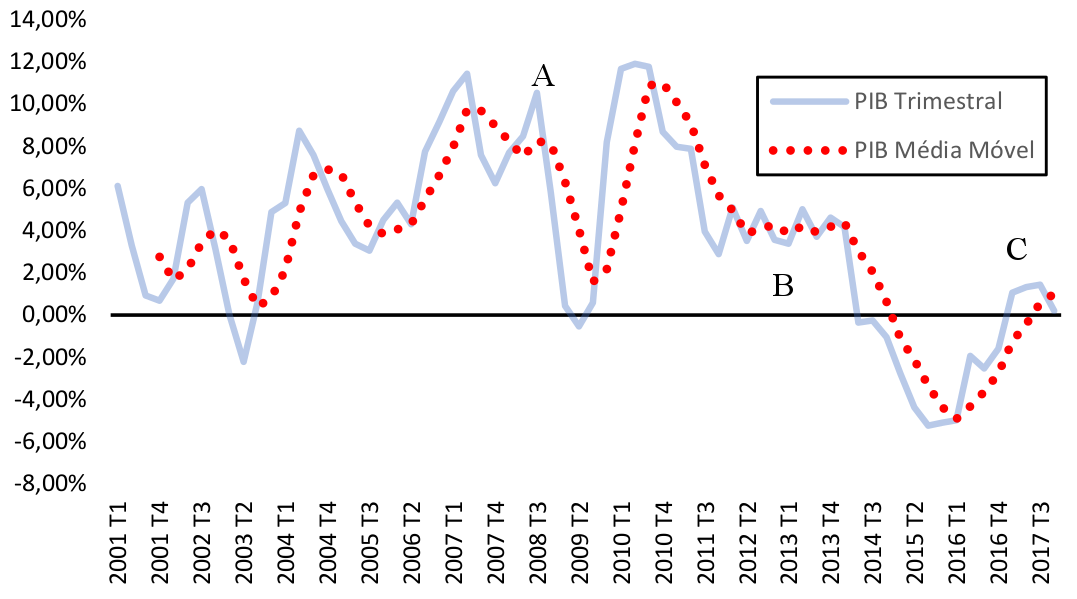
\includegraphics[width=\textwidth]{PIB_FAPESP}
\end{center}
\caption*{\textbf{Fonte:} Elaboração própria, dados do IPEADATA}
\end{figure}
% TODO Verificar fonte

Como esperado, essa crise está sendo alvo das mais diferentes 
interpretações.
Grosso modo, boa parte da literatura alveja as políticas econômicas como fonte desta desaceleração dinâmica, sejam elas austeras \cite{serrano_demanda_2015}, intervencionistas \cite{barbosa_filho_crise_2017}, estruturais \cite{bacha_saida_2017} ou até mesmo decorrentes das limitações da ossatura do Estado desenvolvimentista \cite{carneiro_economia_2017}. Com isso, indicam-se as fragilidades do padrão de crescimento brasileiro decorrentes das medidas inadequadas de política econômica, mas argumenta-se aqui que existem fatores estruturais que devem ser considerados.

Esta pesquisa, portanto, tem um aspecto mais generalizante e tenta dar conta dos movimentos referentes às mudanças redistributivas tal como em \textcite{serrano_conflito_2018}. Vale notar que esta investigação não pretende dar uma explicação para o caso brasileiro recente, mas sim, contribuir para a compreensão deste episódio à luz da teoria monetária da distribuição de \textcite{pivetti_essay_1992}.

Deste modo, procura-se evidenciar alguns elementos que esclarecem a trajetória da economia brasileira tendo em vista transformação distributiva observada. Os gráficos da figura \ref{Distri} apresentam um retrato da economia brasileira em termos da distribuição de renda.


\begin{figure}[H] % Inicia o ambiente de figuras
	\begin{center}
	\caption{Retrato distributivo no Brasil (2005-2015)}
	\label{Distri}
	\subfigure[Participação na renda disponível (2006-2015) - percentis selecionados]{ % Começa a incluir a figura fig1.pdf
		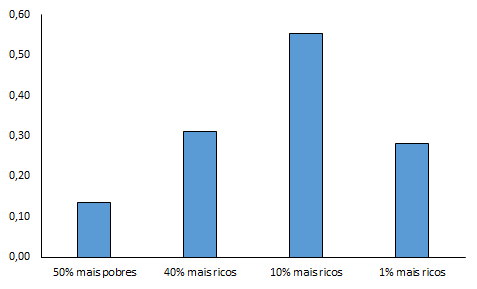
\includegraphics[height=1.8in]{Plot_Part_renda.png}\label{Part}
	} % Termina de incluir a figura fig1.pdf
	\subfigure[Razão entre a renda dos 10\% mais ricos e dos 40\% mais pobres (2006-2014)]{ % Começa a incluir a figura fig2.pdf na mesma linha da figura fig1.pdf
		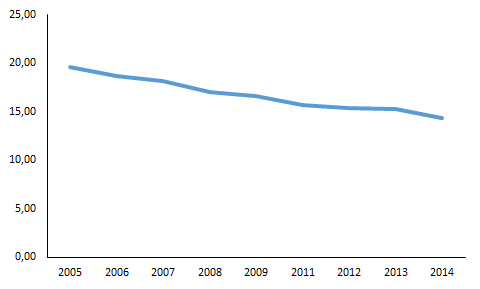
\includegraphics[height=1.8in]{Plot_Percentil_Rel.png}\label{Razao}
	} % Termina de incluir a figura fig2.pdf
	\end{center}
\caption*{\textbf{Fonte:} Elaboração própria, dados do IPEADATA}
% TODO Verificar fonte
\end{figure} % Fecha o ambiente de figuras
% TODO Corrigir labels

O gráfico 2(a) mostra como os estratos mais altos da renda (10\% e 1\% mais ricos) capturaram, em média, maior parte da renda disponível (mais de 60\% ao todo). Desse modo, fica evidente como a distribuição pessoal da renda é bastante concentrada. No entanto, o gráfico 2(b) evidencia as mudanças redistributivas mencionadas anteriormente. Os decis mais ricos detinham uma parcela crescente, mas a taxas decrescentes, da renda ao longo do período. Os mais pobres, por outro lado, tiveram um crescimento na participação relativamente superior aos mais ricos, configurando uma redistribuição da renda à favor dos estrados mais baixos. Portanto, observa-se uma crescente e tênue participação dos mais pobres na renda em detrimento dos mais ricos. 
Sendo assim, procura-se investigar como essas transformações na economia brasileira afetaram o crescimento econômico.
Por fim, dado este panorama, a seção \ref{OBJ} irá apresentar os objetivos pretendidos com esta pesquisa.
